\documentclass[letterpaper,12pt,oneside]{book}
%\usepackage[a4paper,includeall,bindingoffset=0cm,margin=2cm,marginparsep=0cm,marginparwidth=0cm]{geometry}
%\usepackage[top=1in, left=0.9in, right=1.25in, bottom=1in]{geometry}
%\usepackage{bachelorstitlepageUNAM}
\usepackage{ragged2e}
\usepackage{times}
\usepackage{listings}
\usepackage{xcolor}
%\usepackage{background}
\usepackage[utf8]{inputenc}
\usepackage{url}
\usepackage[T1]{fontenc}
\usepackage[spanish,es-nodecimaldot,es-tabla]{babel}
\usepackage{graphicx}
\usepackage{tikz}
\usepackage{tocloft}
\graphicspath{{./figs/}}
\usepackage{setspace}
\usepackage{comment}
\usepackage{hyperref}
\urlstyle{same}
\hypersetup{
   colorlinks=true,
   urlcolor=cyan,
   linkcolor=black,
   citecolor=black,
   filecolor=magenta,
   pdftitle={Sharelatex Example},
   pdfpagemode=FullScreen,
}
\usepackage[natbibapa]{apacite}
%\usepackage[round]{natbib}

%\renewcommand\cftsecpresnum{\S}
%\renewcommand\cftsubsecpresnum{\S}

%%%%%%%%%%%%%%%%%%%%%%%%%%%%%

% Modificación de la plantilla original de esta url: 
% https://es.overleaf.com/latex/templates/tesis-unam-ingenieria-energia/kfffjrxcckdp

% Adaptada por Carlos Rodríguez Díaz para el CIC IPN.
% Cualquier sugerencia, corrección o comentario a: amnet04@gmail.com

% A continuación los comentarios de la plantilla original:

% Comparto una plantilla para la PORTADA que us\'e en mi t\'esis
% basada en el dise\~no gen\'erico que se usa en la Facultad de Ciencias
% Para usarlo \'unicamente aseg\'urate de tener la l\'inea
% \usepackage{bachelorstitlepageUNAM} y el archivo bachelorstitlepageUNAM.sty en el mismo directorio de trabajo.
% y los campos (sin signo %) :
%\author{Nombre del Alumno}
%\title{T\'itulo de la tesis}
%\faculty{Facultad}
%\degree{Grado que obtienes}
%\supervisor{ Tutor}
%\cityandyear{Ciudad y anio}
%\logouni{nombredelescudodelaunamsinespacios}
%\logofac{NombreDeLaImagenDelEscudodeTuFacultadSinEspacios}
% Para sugerencias y comentarios: DM en twitter.com/sglvgdor
% Subir\'e mas adelante la plantilla para maestr\'ia
%%%%%%%%%%%%%%%%%%%%%%%%%%%%%


\begin{document}

\frontmatter
            \begin{titlepage}
  \thispagestyle{empty}
  \begin{minipage}[c][0.17\textheight][c]{0.25\textwidth}
    \begin{center}
      
\includegraphics[ height=4cm]{Images/logo-ipn.png}
    \end{center}
  \end{minipage}
  \begin{minipage}[c][0.195\textheight][t]{0.75\textwidth}
    \begin{center}
      \vspace{0.3cm}
             {\color{red}\textsc{\large Instituto Politécnico Nacional} }\\[0.5cm]
             \vspace{0.3cm}
                    {\color{purple}\hrule height2.5pt}
                    \vspace{.2cm}
                           {\color{purple}\hrule height1pt}
                           \vspace{.8cm}
                           \textsc{Escuela Superior de Cómputo }\\[1cm] %
    \end{center}
  \end{minipage}
  \begin{minipage}[c][0.81\textheight][t]{0.25\textwidth}
    \vspace*{5mm}
    \begin{center}
      \hskip2.0mm
             {\color{red}\vrule width1pt height13cm }
             \vspace{5mm}
             \hskip2pt
                 {\color{red}\vrule width2.5pt height13cm}
                 \hskip2mm
                     {\color{red}\vrule width1pt height13cm} \\
                     \vspace{5mm}
                     
\includegraphics[height=3.0cm]{Images/CIC.png}
    \end{center}
  \end{minipage}
  \begin{minipage}[c][0.81\textheight][t]{0.75\textwidth}
    \begin{center}
      \vspace{1cm}

      {\color{red}{\large\scshape Titulo del Reporte }}\\[.2in]

      \vspace{2cm}            

      \textsc{\LARGE P\hspace{0.5cm}R\hspace{0.5cm}O\hspace{0.5cm}G\hspace{0.5cm}R\hspace{0.5cm}A\hspace{0.5cm}M\hspace{0.5cm}A\hspace{0.5cm}}\\[1cm]
      \textsc{\LARGE M\hspace{0.5cm}Á\hspace{0.5cm}Q\hspace{0.5cm}U\hspace{0.5cm}I\hspace{0.5cm}N\hspace{0.5cm}A\hspace{0.5cm}\hspace{0.5cm}D\hspace{0.5cm}E}\\[1cm]
      \textsc{\LARGE\hspace{0.5cm}T\hspace{0.5cm}U\hspace{0.5cm}R\hspace{0.5cm}I\hspace{0.5cm}N\hspace{0.5cm}G}
      \\[1cm]
      \textsc{\large que para obtener un 10 en el reporte:}\\[0.2cm]
     % \textsc{\large XXXX XXXX XXXXX}\\[0.5cm]
      
      {\color{red}\textsc{\large presenta:}}\\[0.2cm]
      \textsc{\large {Connor Urbano Mendoza}}\\[1cm]          

      \vspace{0.5cm}

      {\large\scshape 
        {\color{red}Docente:}\\[0.3cm] {Juárez Martínez Genaro}}\\[.2in]

      \vspace{1cm}

      \large{Estados Unidos Mexicanos\\ 
        Ciudad de México\\
        2023}
    \end{center}
  \end{minipage}
\end{titlepage}
%---------------------------------
\tableofcontents
\listoffigures
%\chapter{Notación}


\chapter{Introducción}
En esta práctica, vamos a trabajar con una máquina de Turing diseñada para reconocer el lenguaje {$0^n$$1^n$ | n >=1}, es decir, cadenas formadas por una secuencia de ceros seguida por una secuencia de unos, donde el número de ceros y unos es el mismo y mayor o igual a uno. Esta máquina de Turing se basa en el libro de John Hopcroft, en el ejercicio 8.2 de la segunda edición.\newline

La máquina de Turing que construiremos seguirá un proceso específico para transformar la entrada dada. Comenzando desde el extremo izquierdo de la cinta, la máquina cambiará secuencialmente los ceros por la letra X y se moverá hacia la derecha, pasando por encima de cualquier cero o letra Y que encuentre, hasta que encuentre un uno. En ese momento, cambiará el uno por la letra Y y se moverá hacia la izquierda, pasando sobre cualquier letra Y o cero hasta que encuentre una X. En esta situación, buscará un cero colocado inmediatamente a la derecha y, si lo encuentra, lo cambiará por una X y repetirá el proceso, cambiando el uno correspondiente por una Y.\newline

Si la entrada no cumple con el patrón $0^n$$1^n$, la máquina de Turing se detendrá sin aceptar la cadena. Sin embargo, si la máquina logra cambiar todos los ceros por X en la misma iteración en la que cambia el último uno por una Y, entonces se determina que la entrada es de la forma $0^n$$1^n$ y la máquina la acepta.\newline

En esta práctica, implementaremos la máquina de Turing en Python, permitiendo que el usuario ingrese una cadena o generando una automáticamente. El programa generará un archivo de texto como salida, que contendrá las descripciones instantáneas en cada paso de la computación. También animaremos la máquina de Turing para cadenas de longitud menor o igual a 10 caracteres.\newline

A continuación, se presenta el código de la máquina de Turing y se proporciona en el reporte, junto con el archivo fuente del código.\newline

Esta práctica se basa en conceptos de teoría de la computación, específicamente en el estudio de gramáticas formales y sus derivaciones. El propósito es aplicar estos conceptos para implementar un programa que pueda procesar y generar cadenas válidas según una gramática específica.\newline

La tabla de transiciones a utilizar en el desarrollo de esta práctica es:\newline

\begin{figure}[h]
%\begin{minipage}{0.3\textwidth}
    \begin{center}
    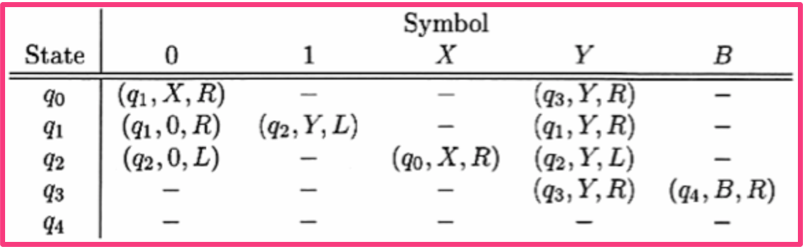
\includegraphics[width=1\linewidth]{Images/tabla.png}
    \end{center}
%\end{minipage}
\caption{Tabla de estados para el problema.}
\label{fig:imagen}
\end{figure}


\mainmatter
\chapter{Desarrollo}
\lstset{
    language=C,
    basicstyle=\ttfamily\small\color{black},
    numbers=left,
    numberstyle=\tiny,
    stepnumber=1,
    numbersep=8pt,
    backgroundcolor=\color{white},
    showspaces=false,
    showstringspaces=false,
    showtabs=false,
    frame=single,
    rulecolor=\color{magenta},
    tabsize=2,
    captionpos=b,
    breaklines=true,
    breakatwhitespace=false,
    title=\lstname,
    escapeinside={\%*}{*)},
    keywordstyle=\color{blue},
    commentstyle=\color{red},
    stringstyle=\color{orange},
    morecomment=[l][\color{red}]{\#},
    otherkeywords={=,!,<,>,*,+,-,&,|,^,~},
    numbers=left,                   % Coloca los números de línea a la izquierda
    numberstyle=\tiny\color{black}, % Estilo de los números de línea
    stepnumber=1,    % Incremento en el que se muestran los números de línea
    numbersep=8pt
}
\section{Análisis del problema principal}

%\begin{comment}
  %Objetivo: Explicarles a los lectores de computación que entienden
  %los lingüistas de una variación dialectal
%\end{comment}

%Citar a \cite{deSaussure1945}, Coseriu y Montes:

Al resolver el problema de la máquina de Turing y programarla, se deben considerar los siguientes aspectos:\newline
\begin{enumerate}
    \item Definición del lenguaje: Es importante comprender claramente el lenguaje que se desea reconocer con la máquina de Turing. En el caso específico mencionado, el lenguaje es {$0^n$$1^n$ | n ≥ 1}, lo que significa que debe haber una secuencia de ceros seguida de una secuencia igual de unos.\newline

    \item Tabla de transiciones: Se debe crear una tabla de transiciones que defina las reglas para cambiar de un estado a otro en función del símbolo leído en la cinta. La tabla de transiciones debe contener información sobre el estado actual, el símbolo leído, el estado siguiente, el símbolo a escribir en la cinta y la dirección en la que se moverá el cabezal.\newline
    
    \item Implementación de los estados y transiciones: Es necesario implementar los diferentes estados de la máquina de Turing y programar las transiciones correspondientes según las reglas establecidas en la tabla de transiciones. Esto implica manejar correctamente el cambio de estado, la lectura y escritura de símbolos en la cinta, y el movimiento del cabezal.\newline
    
    \item Manejo de la entrada y salida: Se debe tener en cuenta cómo se proporcionará la entrada a la máquina de Turing y cómo se mostrarán los pasos de computación en la salida. Puede ser necesario leer la cadena definida por el usuario o generar una automáticamente, y registrar las descripciones instantáneas en cada paso en un archivo de texto.\newline
    
    \item Validación y aceptación: Durante la ejecución del programa de la máquina de Turing, se deben verificar las condiciones de aceptación o rechazo de una entrada. En el caso mencionado, la máquina de Turing aceptará si todos los ceros se han cambiado por X y el último uno se ha cambiado por Y en la misma iteración. Si la entrada no cumple con estas condiciones, la máquina de Turing se detendrá sin aceptar.\newline
\end{enumerate}


El análisis de estos problemas, facilita la programación de la máquina de Turing y se asegura una solución adecuada para el problema planteado. \newline


\section{Límites del problema}%seccion2
Los límites del problema establecidos por el profesor e implícitamente en esta práctica son los siguientes:\newline
\begin{enumerate}
    \item Longitud máxima de la cadena: El programa debe ser capaz de recibir una cadena definida por el usuario o generada automáticamente por la máquina, pero la longitud de la cadena no debe exceder los 1000 caracteres. Esto implica que la máquina de Turing debe estar diseñada y programada para manejar cadenas de hasta 1000 caracteres como máximo.\newline

    \item Animación con cadenas menores a 10 caracteres: Para facilitar la comprensión y visualización del funcionamiento de la máquina de Turing, se debe animar su ejecución con cadenas que tengan una longitud igual o menor a 10 caracteres. Esto implica que se deberá realizar una representación gráfica o visual de la cinta y el cabezal, mostrando los movimientos y cambios de símbolos durante la ejecución de la máquina.\newline
    
    \item Salida en archivo de texto: La salida del programa debe ser redirigida a un archivo de texto. Es decir, en cada paso de la computación, se debe generar una descripción instantánea que se registrará en un archivo de texto. Esta salida permitirá seguir el proceso de ejecución de la máquina de Turing y analizar su comportamiento.\newline
    
\end{enumerate}
Estos límites establecidos por el profesor definen las restricciones específicas para la implementación y presentación de la solución del problema de la máquina de Turing.\newline

\section{Estrategia para atacar el problema}
%inicio
 A continuación, se describen las estrategias utilizadas para solucionar el problema de la máquina de Turing:\newline
\begin{enumerate}
    \item EInterfaz gráfica: El código utiliza la biblioteca pygame para crear una ventana y dibujar los elementos gráficos necesarios, como los cuadros de la cinta y los botones.\newline

    \item Representación de la cinta: La cinta de la máquina de Turing se representa como una lista en el código, donde cada elemento de la lista corresponde a un símbolo en la cinta.\newline
    
    \item Reglas de transición: Las reglas de transición de la máquina de Turing se definen en una lista llamada $"$rules$"$. Cada regla se representa como una tupla de la forma (estado\_actual, simbolo\_actual) -> (nuevo\_simbolo, dirección, nuevo\_estado).\newline
    
    \item Ejecución de la máquina de Turing: La función turing\_M se encarga de ejecutar la máquina de Turing. Recibe los parámetros iniciales, como el estado inicial, el símbolo blanco, las reglas de transición y la cinta. Luego, sigue las reglas de transición para procesar la cinta hasta alcanzar un estado final.\newline
\end{enumerate}


\section{Implementación} 
Aquí se explica qué hace cada parte del código:\newline
\\
\begin{enumerate}
    \item Se importan los módulos necesarios: random para generar números aleatorios y pygame para la creación de la interfaz gráfica del juego.\newline

    \item Se inicializa el módulo pygame mediante pygame.init() para poder utilizar sus funciones y recursos.\newline
    
    \item Se definen las variables WIDTH y HEIGHT para el ancho y altura de la ventana del juego.\newline
    
    \item Se crea la ventana del juego con las dimensiones especificadas en WIDTH y HEIGHT mediante pygame.display.set\_mode((WIDTH, HEIGHT)). Además, se establece el título de la ventana como 'Maquina de turing' mediante pygame.display.set\_caption('Maquina de turing').\newline
    
    \item Se crean dos objetos Font de pygame para definir el tipo y tamaño de la fuente utilizada en el juego.\newline
    
    \item Se crea un objeto Clock de pygame llamado timer para controlar la velocidad de actualización del juego.\newline
    
    \item Se define la variable fps para establecer la cantidad de fotogramas por segundo a los que se actualizará el juego.\newline
    
    \item Se definen las variables ubicacion, turn\_step y selection, que se utilizan para almacenar información y controlar los turnos en el juego.\newline
    
    \item Se define la función dibujar\_boton() que dibuja un botón en la pantalla del juego utilizando la función pygame.draw.rect(). El botón se muestra como un rectángulo verde con el texto 'Siguiente' en el centro. La función devuelve un objeto Rect de pygame que representa el área del botón.\newline
    
    \item Se define la función mostrar\_transiciones(recorrido, estado) que se encarga de mostrar las transiciones de la Máquina de Turing en la pantalla del juego. La función recibe dos argumentos: recorrido, que es una cadena que representa las transiciones realizadas, y estado, que es una cadena que representa el estado actual de la Máquina de Turing. La función utiliza varias operaciones de pygame para dibujar las transiciones en la pantalla, como dibujar rectángulos, texto y cargar imágenes.\newline
     \begin{enumerate}
        \item Esta función se encarga de mostrar las transiciones de la Máquina de Turing en la pantalla del juego.
        \item Recibe dos argumentos: recorrido, que es una cadena que representa las transiciones realizadas, y estado, que es una cadena que representa el estado actual de la Máquina de Turing.\newline
        \item La función recorre cada transición del recorrido y las muestra en la pantalla.\newline
        \item Para cada transición, se dibuja un cuadro en la posición correspondiente en la pantalla y se muestra el valor de la transición en el centro del cuadro.\newline
        \item Si una transición comienza con [, significa que es una transición especial. En este caso, se realizan acciones adicionales, como cambiar el color del cuadro, agregar marcadores o mostrar el estado actual de la Máquina de Turing.\newline
        \item Para mostrar el estado actual, se utiliza la función blit() de pygame para pegar el texto del estado en la posición adecuada dentro del cuadro.\newline
        \item Al final de la función, se muestra en la pantalla el conjunto de cuadros con las transiciones y los elementos especiales.
     \end{enumerate}
    
    \item Se define la función dibujar\_tablero() que se encarga de dibujar el tablero de la Máquina de Turing en la pantalla del juego. La función utiliza operaciones de pygame para dibujar los cuadros del tablero en la pantalla.\newline
    \begin{enumerate}
        \item Esta función se encarga de dibujar el tablero de la Máquina de Turing en la pantalla del juego. Utiliza operaciones de pygame para dibujar una cuadrícula de cuadros en la pantalla que representan el tablero.\newline
        \item Cada cuadro se dibuja como un rectángulo con un tamaño determinado y un color específico.\newline
        \item La función itera sobre los cuadros del tablero y los dibuja en la pantalla.\newline
        \item Además de dibujar los cuadros, se añade un borde de color negro alrededor de cada cuadro para resaltarlo visualmente.\newline
        \item Al finalizar la función, se muestra en la pantalla el tablero completo con sus cuadros y bordes.\newline
    \end{enumerate}
\end{enumerate}

El fragmento de código que acabamos de explicar pertenece a la figura 1.1.  Observar figura 1.1.\newline

\begin{lstlisting}
#Teoria de la computacion
#Maquina de turing
#Alumno: Connor Urbano Mendoza
import random
import pygame

pygame.init() #Acceso al paquete pygame
#Ancho
WIDTH = 1300
#Altura
HEIGHT = 700
screen = pygame.display.set_mode((WIDTH,HEIGHT)) #Tamanio de ventana a imprimir
pygame.display.set_caption('Maquina de turing')
font = pygame.font.Font('freesansbold.ttf',20)#Tipo de fuente 1 del juego
big_font= pygame.font.Font('freesansbold.ttf',50)#Tipo de fuente 2 del juego
timer = pygame.time.Clock()#velocidad de actualizacion de nuestro juego a 60 fps
fps=60

#Variables e imagenes del juego
ubicacion = ['recuadro']

#Variables de turnos cambiantes
turn_step = 0
selection= 100
#Cargar imagenes en juego
cuadro = pygame.image.load('C:\\Users\\soyco\\OneDrive\\Documents\\ESCOM\\sem4\\Teoria\\P2\\turing\\img\\cuadro.png')
cuadro = pygame.transform.scale(cuadro,(101,101))

cuadrado = [cuadro]

lista_piezas = ['recuadro']

#ver variables/contador flash
boton_presionado = False

def dibujar_boton():
    boton_width = 150
    boton_height = 45
    boton_x = (WIDTH - boton_width) // 2
    boton_y = (HEIGHT - boton_height - 20)-100

    # Dibujar el botón como un rectángulo en la pantalla
    boton_rect=pygame.Rect(boton_x, boton_y, boton_width, boton_height)
    pygame.draw.rect(screen, (0, 255, 0), (boton_x, boton_y, boton_width, boton_height))
    texto = font.render("Siguiente", True, (0, 0, 0))
    texto_rect = texto.get_rect(center=(boton_x + boton_width // 2, boton_y + boton_height // 2))
    screen.blit(texto, texto_rect)
    return boton_rect
   
#Funcion para dibujar el contenido de la maquina de turing
def mostrar_transiciones(recorrido,estado):
    
    #recorrido="X,0,0,1,[1],1,1,1,"
    #estado="q2"
    cuadro_size = 100  # Tamaño de cada cuadro del tablero
    x = 0
    y = 255
    
    font = pygame.font.Font(None, 100)  # Fuente y tamaño del número de casilla

    transiciones = recorrido.split(',')  # Obtener las transiciones del recorrido

    for i, transicion in enumerate(transiciones):
        if i >= 12:
            break  # Salir del bucle si se han mostrado todas las transiciones posibles
        x = x + 100
        if transicion.startswith('['):
            # Realizar alguna acción especial para la transición que comienza con '['
            # Por ejemplo, cambiar el color del recuadro o agregar un marcador adicional
            numero_texto = font.render("^", True, 'yellow')  # Crear superficie de texto con la transición
            numero_rect = numero_texto.get_rect(center=((x, y+110)))  # Posición del texto en el centro del recuadro
            screen.blit(numero_texto, numero_rect)  # Pegar el texto en la pantalla
            numero_texto = font.render("|", True, 'yellow')  # Crear superficie de texto con la transición
            numero_rect = numero_texto.get_rect(center=((x, y+120)))  # Posición del texto en el centro del recuadro
            screen.blit(numero_texto, numero_rect)  # Pegar el texto en la pantalla
            numero_texto = font.render(estado, True, 'yellow')  # Crear superficie de texto con la transición
            numero_rect = numero_texto.get_rect(center=((x, y+190)))  # Posición del texto en el centro del recuadro
            screen.blit(numero_texto, numero_rect)  # Pegar el texto en la pantalla
            index=lista_piezas.index('recuadro')
            screen.blit(cuadrado[index],(x-50,y-55))
            
        numero_texto = font.render(transicion, True, 'black')  # Crear superficie de texto con la transición
        numero_rect = numero_texto.get_rect(center=((x, y)))  # Posición del texto en el centro del recuadro
        screen.blit(numero_texto, numero_rect)  # Pegar el texto en la pantalla
 
#Funcion para dibujar tablero
def dibujar_tablero():
    cuadro_size = 100  # Tamaño de cada cuadro del tablero
    tablero_width = 12 * cuadro_size  # Ancho total del tablero
    tablero_height = 1 * cuadro_size  # Altura total del tablero
    tablero_x = (WIDTH - tablero_width) // 2  # Posición X para centrar el tablero
    tablero_y = ((HEIGHT - tablero_height) // 2 )-200 # Posición Y para centrar el tablero

    for i in range(12):  # Iterar 12 veces para un tablero de 1x12
        columna = i % 12
        fila = 1
        x = tablero_x + columna * cuadro_size
        y = tablero_y + fila * cuadro_size
        if fila % 2 == 0:
            color = 'white' if columna % 2 == 0 else (226, 255, 255)
        else:
            color = (226, 255, 255) if columna % 2 == 0 else 'white'
        pygame.draw.rect(screen, color, [x, y, cuadro_size, cuadro_size])
        pygame.draw.rect(screen, 'black', [x, y, cuadro_size, cuadro_size], 2)  # Agregar borde de color 
       
 
\end{lstlisting}
\begin{figure}[h]
\begin{center}
\end{center}
\caption{Inicio del código, librería random y funciones básicas.}
\label{fig:imagen}
\end{figure}

La función turing\_M() es una implementación de una Máquina de Turing que realiza una simulación y guarda los resultados en un archivo de texto. A continuación, explicaré en detalle cómo funciona y qué hace cada parte del código:\newline
\begin{enumerate}
    \item Parámetros de la función:\newline
    \begin{enumerate}
        \item state: Representa el estado actual de la Máquina de Turing.\newline
        \item blank: Es el símbolo en blanco del alfabeto de la cinta.\newline
        \item rules: Es una lista de reglas de transición que define cómo la Máquina de Turing se mueve y cambia de estado.\newline
        \item tape: Es la cinta de la Máquina de Turing, representada como una lista de símbolos.\newline
        \item final: Representa el estado final o de aceptación de la Máquina de Turing.\newline
        \item pos: Es la posición actual del cabezal de lectura/escritura en la cinta.\newline
    \end{enumerate}
    
    \item Inicialización y validación de parámetros:\newline
    \begin{enumerate}
        \item La función asigna el estado inicial st con el valor de state.\newline
        \item Si la cinta está vacía (tape es una lista vacía), se asigna un símbolo en blanco (blank) como único elemento de la cinta.\newline
        \item Se verifica y corrige la posición pos del cabezal de lectura/escritura. Si es negativa, se ajusta al tamaño de la cinta.\newline
        \item Si la posición está fuera del rango válido de la cinta, se muestra un mensaje de error y se termina el programa con SystemExit(1).\newline
    \end{enumerate}
    
    \item Preparación de las reglas de transición:\newline
    \begin{enumerate}
        \item La función asigna el estado inicial st con el valor de state. La variable rules se transforma de una lista de reglas de transición a un diccionario para facilitar el acceso y búsqueda.\newline
        \item Cada regla de transición de la forma (s0, v0, v1, dr, s1) se convierte en una entrada del diccionario donde la clave es una tupla (s0, v0) y el valor es una tupla (v1, dr, s1).\newline
        

    \end{enumerate}
    
    \item Ciclo principal de ejecución:\newline
    \begin{enumerate}
        \item El bucle principal se ejecuta continuamente hasta que se alcanza el estado final (final) o si no se encuentra una regla de transición para el estado y símbolo actuales.\newline
        \item En cada iteración del bucle, se guarda el estado actual (st) y la configuración de la cinta en un archivo de texto especificado (turing.txt). Cada línea del archivo contiene el estado y los símbolos de la cinta separados por comas. El símbolo en la posición actual del cabezal de lectura/escritura se muestra entre corchetes.\newline
        \item Si se alcanza el estado final, se muestra el mensaje 'Cadena válida' y se rompe el bucle.\newline
        \item Si no se encuentra una regla de transición para el estado y símbolo actuales, se muestra el mensaje "Cadena inválida" y se rompe el bucle.\newline
    \end{enumerate}
    
    \item Ejecución de las reglas de transición:\newline
    \begin{enumerate}
        \item Si se encuentra una regla de transición para el estado y símbolo actuales, se obtiene la tupla (v1, dr, s1) correspondiente.\newline
        \item Se actualiza el símbolo de la cinta en la posición actual (pos) con el nuevo símbolo v1.\newline
        \item Luego, se mueve el cabezal de lectura/escritura según la dirección indicada por dr. Si es 'left', se mueve hacia la izquierda disminuyendo pos. Si es 'right', se mueve hacia la derecha aumentando pos. Si la posición está fuera del rango de la cinta, se agrega un símbolo en blanco al final o al principio de la cinta, según corresponda.\newline
        \item Luego, se mueve el cabezal de lectura/escritura según la dirección indicada por dr. Si es 'left', se mueve hacia la izquierda disminuyendo pos. Si es 'right', se mueve hacia la derecha aumentando pos. Si la posición está fuera del rango de la cinta, se agrega un símbolo en blanco al final o al principio de la cinta, según corresponda.\newline
        \item El estado actual (st) se actualiza con el nuevo estado s1 obtenido de la regla de transición.\newline
    \end{enumerate}
     Observar figura 1.2.
\end{enumerate}
\begin{lstlisting}
def turing_M (state = None, #estados de la maquina de turing
              blank = None, #simbolo blanco de el alfabeto dela cinta
              rules = [],   #reglas de transicion
              tape = [],    #cinta
              final = None,  #estado valido y/o final
              pos = 0):#posicion siguiente de la maquina de turing

    st = state
    if not tape: tape = [blank]
    if pos <0 : pos += len(tape)
    if pos >= len(tape) or pos < 0 : 
        print("Se inicializa mal la posicion")
        SystemExit(1)
    
    rules = dict(((s0, v0), (v1, dr, s1)) for (s0, v0, v1, dr, s1) in rules)
    """
        Estado	Símbolo leído	Símbolo escrito	       Mov. 	Estado sig.
        qn(s0)  1,0,X,Y,B(v0)	  1,0,X,Y,B(v1)       R o L(dr)	   qn(s1)
    """
    while True:
        with open('C:\\Users\\soyco\\OneDrive\\Documents\\ESCOM\\sem4\\Teoria\\P2\\turing\\output\\turing.txt', 'a') as archivo:
            archivo.write(st+ '\n')
            #print (st, '\t', end=" ")
            for i, v in enumerate(tape):
                if i==pos: 
                    #print ("[%s]"%(v,),end=" ")
                    archivo.write('['+v+'],')
                else: 
                    #print (v, end=" ")
                    archivo.write(v+',') 
            #print()
            archivo.write('\n')
            if st == final: 
                print("Cadena valida.")
                break
            if (st, tape[pos]) not in rules: 
                print("Cadena invalida.")
                break
            
            (v1,dr,s1) = rules [(st, tape[pos])]
            tape[pos]=v1 #rescribe el simbolo de la cinta
    
    #movimiento del cabezal
        if dr == 'left':
            if pos > 0: pos -= 1
            else: tape.insert(0, blank)
        if dr == 'right':
            pos += 1
            if pos >= len(tape): tape.append(blank)
        st = s1
\end{lstlisting}
\begin{figure}[h]
\begin{center}
\end{center}
\caption{Función de recorrido de turing.}
\label{fig:imagen}
\end{figure}
\newpage

La función turing MG hace exactamente lo mismo que la primera, solo que el formato de guardado para el archivo de salida es diferente, esto se hace debido a que en la primera maquina está destinada a casos menores a 10 (donde se requiere una animación). Sin embargo, para casos muy grandes y sin animación lo mejor es guardar la información de manera lineal en el archivo de salida, de esta manera no desperdiciamos tantos recursos de memoria. Observar figura 1.3.\newline


\begin{lstlisting}
ef turing_MG (state = None, #estados de la maquina de turing
              blank = None, #simbolo blanco de el alfabeto dela cinta
              rules = [],   #reglas de transicion
              tape = [],    #cinta
              final = None,  #estado valido y/o final
              pos = 0):#posicion siguiente de la maquina de turing

    st = state
    if not tape: tape = [blank]
    if pos <0 : pos += len(tape)
    if pos >= len(tape) or pos < 0 : 
        print("Se inicializa mal la posicion")
        SystemExit(1)
    
    rules = dict(((s0, v0), (v1, dr, s1)) for (s0, v0, v1, dr, s1) in rules)
    """
        Estado	Símbolo leído	Símbolo escrito	       Mov. 	Estado sig.
        qn(s0)  1,0,X,Y,B(v0)	  1,0,X,Y,B(v1)       R o L(dr)	   qn(s1)
    """
    while True:
        with open('C:\\Users\\soyco\\OneDrive\\Documents\\ESCOM\\sem4\\Teoria\\P2\\turing\\output\\turing.txt', 'a') as archivo:
            archivo.write('|-'+st+ '->')
            #print (st, '\t', end=" ")
            for i, v in enumerate(tape):
                if i==pos: 
                    #print ("[%s]"%(v,),end=" ")
                    archivo.write('['+v+'],')
                else: 
                    #print (v, end=" ")
                    archivo.write(v+',') 
            #print()
            if st == final: 
                print("Cadena valida.")
                break
            if (st, tape[pos]) not in rules: 
                print("Cadena invalida.")
                break
            
            (v1,dr,s1) = rules [(st, tape[pos])]
            tape[pos]=v1 #rescribe el simbolo de la cinta
    
    #movimiento del cabezal
        if dr == 'left':
            if pos > 0: pos -= 1
            else: tape.insert(0, blank)
        if dr == 'right':
            pos += 1
            if pos >= len(tape): tape.append(blank)
        st = s1

\end{lstlisting}
\begin{figure}[h]
\begin{center}
\end{center}
\caption{Función de turing MG para casos grandes.}
\label{fig:imagen}
\end{figure}
Esta parte de código realiza las siguientes acciones:\newline
\begin{enumerate}
    \item Abre el archivo "turing.txt" en modo de escritura ('w') utilizando la sentencia with open('C:/ Users/ soyco/ OneDrive/ Documents/ ESCOM/ sem4/ Teoria/ P2/ turing/ output/ turing.txt', 'w') as archivo. La declaración with garantiza que el archivo se cerrará correctamente después de su uso.\newline
    \item La sentencia pass se utiliza para indicar que no se realiza ninguna acción en este bloque de código. Es un marcador de posición que se utiliza cuando se requiere sintácticamente un bloque de código, pero no se desea ejecutar ninguna instrucción.\newline
    \item Se imprime 'Maquina de turing' en la consola utilizando la función print().\newline
    \item Se imprime el menú en la consola utilizando la función print():\newline
    \item Se solicita al usuario que elija una opción ingresando un número utilizando la función input(). El valor ingresado se asigna a la variable option.\newline
    Si la opción seleccionada es '1', se ejecuta el siguiente bloque de código:\newline
    \begin{enumerate}
        \item Se solicita al usuario que ingrese una cadena menor a 11 caracteres utilizando la función input(). El valor ingresado se asigna a la variable input\_string.\newline
        \item Se llama a la función turing\_M() con los siguientes argumentos: a) state = 'q0': estado inicial de la máquina de Turing. b) blank = 'B': símbolo blanco del alfabeto de la cinta. c) tape = list(input\_string): inserta los elementos de la cadena en la cinta como una lista. d) final = 'q4': estado válido y/o final. e) rules: reglas de transición representadas como una lista de listas de cadenas divididas por espacios.\newline
        \item Después de la llamada a turing\_M(), se anima la máquina de Turing mediante un ciclo while.\newline
        \item Se lee el contenido del archivo "turing.txt" utilizando la sentencia with open('C:/ Users/ soyco/ OneDrive/ Documents/ ESCOM/ sem4/ Teoria/ P2/ turing/ output/ turing.txt', 'r') as archivo: y se almacena en la variable lineas.\newline
        \item Se ejecuta un ciclo while que se repetirá mientras la variable run sea verdadera.\newline
        \item Dentro del ciclo, se obtiene el estado y el recorrido de la máquina de Turing desde las líneas correspondientes en lineas.\newline
        \item Se llama a las funciones dibujar\_tablero() y dibujar\_boton() para dibujar el tablero y el botón respectivamente en una interfaz gráfica.\newline
        \item Se verifica si se hizo clic en el botón utilizando la función collidepoint() de Pygame.\newline
        \item Se incrementa el valor de leerlinea en 2 para avanzar a las siguientes líneas en lineas.\newline
        \item Finalmente, se actualiza la pantalla y se verifica si se ha cerrado la ventana del programa.\newline
    \end{enumerate}
    Si la opción seleccionada es '2', se ejecuta el siguiente bloque de código:\newline
    \begin{enumerate}
        \item Se genera automáticamente una cadena utilizando la función generate\_auto\_string() y se asigna a la variable input\_string.\newline
        \item Se imprime la cadena generada automáticamente utilizando la función print().\newline
        \item El proceso de animación y verificación se lleva a cabo de manera similar a la opción '1'.\newline
    \end{enumerate}
    \item Si la opción seleccionada no es '1' ni '2', se imprime "Opción inválida. Inténtalo de nuevo." en la consola.\newline
    \item Se imprime "Programa terminó." en la consola.\newline
    
\end{enumerate}

Esta interfaz permite al usuario interactuar con la máquina mediante opciones del menú. Dependiendo de la opción seleccionada, se ingresa manualmente una cadena o se genera automáticamente, y luego se ejecuta la máquina de Turing utilizando las reglas de transición especificadas.  Observar figura 1.4.\newline

\begin{lstlisting}
ef turing_MG (state = None, #estados de la maquina de turing
              blank = None, #simbolo blanco de el alfabeto dela cinta
              rules = [],   #reglas de transicion
              tape = [],    #cinta
              final = None,  #estado valido y/o final
              pos = 0):#posicion siguiente de la maquina de turing

    st = state
    if not tape: tape = [blank]
    if pos <0 : pos += len(tape)
    if pos >= len(tape) or pos < 0 : 
        print("Se inicializa mal la posicion")
        SystemExit(1)
    
    rules = dict(((s0, v0), (v1, dr, s1)) for (s0, v0, v1, dr, s1) in rules)
    """
        Estado	Símbolo leído	Símbolo escrito	       Mov. 	Estado sig.
        qn(s0)  1,0,X,Y,B(v0)	  1,0,X,Y,B(v1)       R o L(dr)	   qn(s1)
    """
    while True:
        with open('C:\\Users\\soyco\\OneDrive\\Documents\\ESCOM\\sem4\\Teoria\\P2\\turing\\output\\turing.txt', 'a') as archivo:
            archivo.write('|-'+st+ '->')
            #print (st, '\t', end=" ")
            for i, v in enumerate(tape):
                if i==pos: 
                    #print ("[%s]"%(v,),end=" ")
                    archivo.write('['+v+'],')
                else: 
                    #print (v, end=" ")
                    archivo.write(v+',') 
            #print()
            if st == final: 
                print("Cadena valida.")
                break
            if (st, tape[pos]) not in rules: 
                print("Cadena invalida.")
                break
            
            (v1,dr,s1) = rules [(st, tape[pos])]
            tape[pos]=v1 #rescribe el simbolo de la cinta
    
    #movimiento del cabezal
        if dr == 'left':
            if pos > 0: pos -= 1
            else: tape.insert(0, blank)
        if dr == 'right':
            pos += 1
            if pos >= len(tape): tape.append(blank)
        st = s1

\end{lstlisting}
\begin{figure}[h]
\begin{center}
\end{center}
\caption{Main del programa.}
\label{fig:imagen}
\end{figure}
\chapter{Análisis de Resultados}
\section{Capturas del programa en ejecución}

A continuación se presenta en orden el proceso de ejecución del programa, donde primeramente se muestra el código en ejecución para la parte de la animación y otro ejemplo más grande donde no se incluye animación.\newline
\newpage

\begin{enumerate}
\item Iniciamos el programa, donde nos pide que introduzcamos una opción en el menú de inicio, seleccionamos opción 1 y luego digitamos '0011' que será nuestra cadena a evaluar. El programa nos indica que la cadena fue evaluada y es valida. Observar la Figura 2.1.

\begin{figure}[h]
%\begin{minipage}{0.3\textwidth}
    \begin{center}
    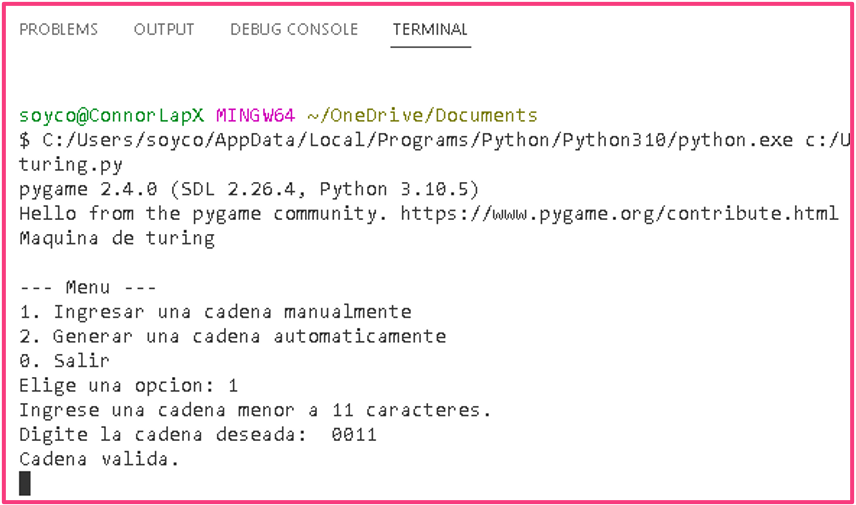
\includegraphics[width=0.8\linewidth]{Images/Cap8.png}
    \end{center}
%\end{minipage}
\caption{Visualización del programa en terminal caso 1.}
\label{fig:imagen}
\end{figure}
\newpage
\item Aquí se puede ver la primera parte de la animación, donde vemos todos las transiciones de la animación, esta animación va cambiando conforme le demos clic al botón 'siguiente'.  Observar la Figura 2.2.\newline
\begin{figure}[h]
%\begin{minipage}{0.3\textwidth}
    \begin{center}
    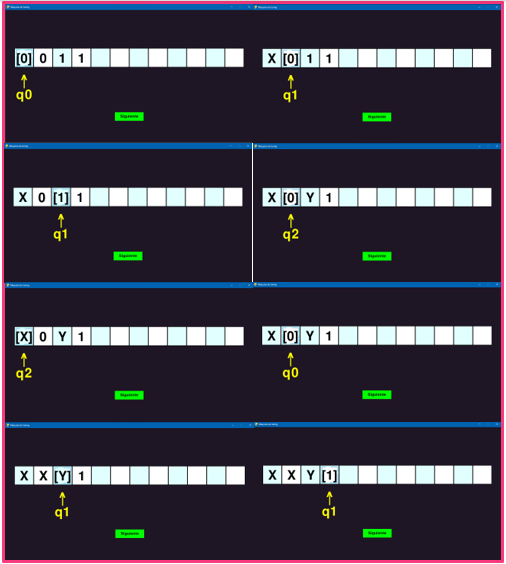
\includegraphics[width=0.8\linewidth]{Images/Cap1.png}
    \end{center}
%\end{minipage}
\caption{Visualización de la primera parte de animaciones.}
\label{fig:imagen}
\end{figure}

\newpage
\item Aquí se puede ver la segunda parte de la animación, donde vemos todos las transiciones de la animación, esta animación va cambiando conforme le demos clic al botón 'siguiente'. En esta última parte podemos ver como llegamos al estado final q4, ya si el programa finaliza. Observar la Figura 2.3.
\begin{figure}[h]
%\begin{minipage}{0.3\textwidth}
    \begin{center}
    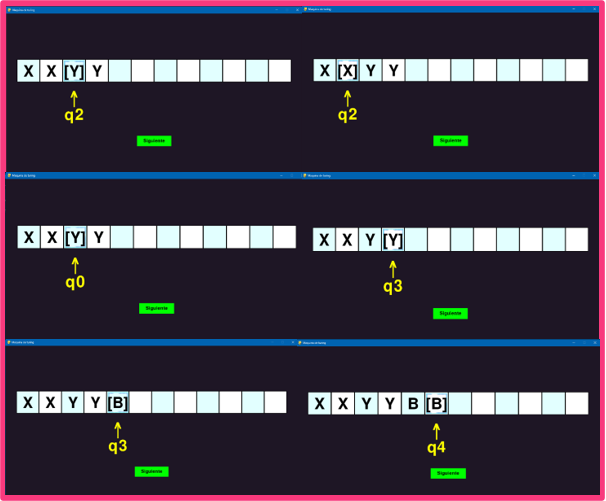
\includegraphics[width=0.8\linewidth]{Images/Cap2.png}
    \end{center}
%\end{minipage}
\caption{Visualización de la segunda parte de animaciones.}
\label{fig:imagen}
\end{figure}

\newpage
\item Aquí podemos ver el archivo de salida turing.txt, que nos mostrara cada paso de las evaluaciones de la máquina de turing. Observar la Figura 2.4.
\begin{figure}[h]
%\begin{minipage}{0.3\textwidth}
    \begin{center}
    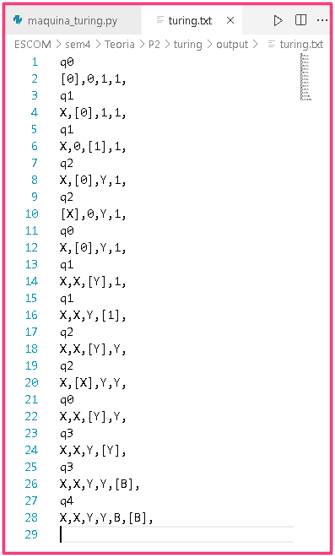
\includegraphics[width=0.5\linewidth]{Images/Cap3.png}
    \end{center}
%\end{minipage}
\caption{Vista del archivo de salida 'turing.txt'.}
\label{fig:imagen}
\end{figure}

\newpage
\item Iniciamos nuevamente el programa, esta vez seleccionamos opción 2 y nos genera una cadena aleatoria, para este caso nos genero una cadena de tamaño 446, posteriormente la evalúa y termina el programa. Observar la figura 2.5.

\begin{figure}[h]
%\begin{minipage}{0.3\textwidth}
    \begin{center}
    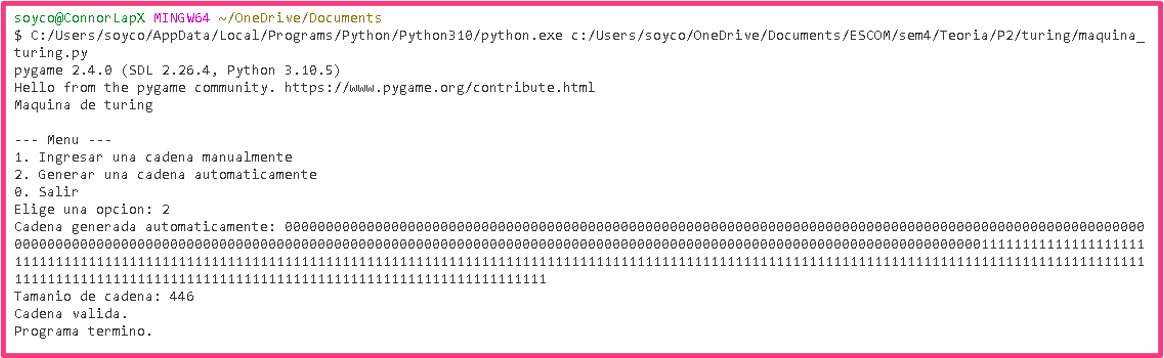
\includegraphics[width=1\linewidth]{Images/Cap4.png}
    \end{center}
%\end{minipage}
\caption{Visualización del programa en terminal caso 2.}
\label{fig:imagen}
\end{figure}

\newpage
\item Vemos que el archivo de salida 'turing.txt' llego a pesar cerca de 90MB, lo que significa que la complejidad del algoritmo incrementa exponencialmente conforme el tamaño de la cadena crece y por ende entre mayor tamaño de cadena, más recursos de memoria serán necesarios. Observar la figura 2.6.

\begin{figure}[h]
%\begin{minipage}{0.3\textwidth}
    \begin{center}
    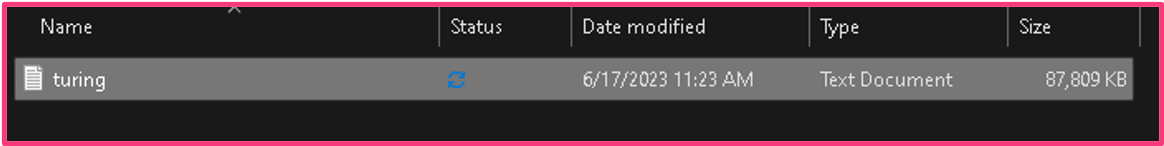
\includegraphics[width=1\linewidth]{Images/Cap5.png}
    \end{center}
%\end{minipage}
\caption{Visualización de memoria utilizada por el archivo para caso 2.}
\label{fig:imagen}
\end{figure}
\newpage
\item Aquí se puede ver el inicio del archivo de 'turing.txt', donde podemos ver que inicia correctamente con el cabezal en la primera posición. Cabe recalcar que se tuvo que hacer uso de una herramienta especial para abrir archivos grandes de información. Observar la figura 2.7.

\begin{figure}[h]
%\begin{minipage}{0.3\textwidth}
    \begin{center}
    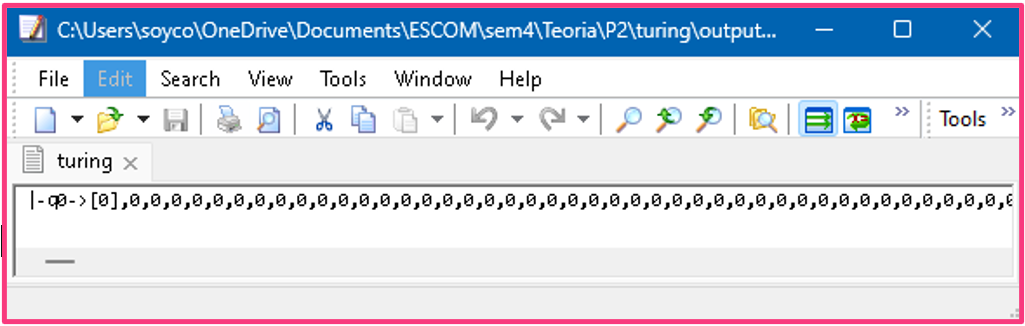
\includegraphics[width=1\linewidth]{Images/Cap6.png}
    \end{center}
%\end{minipage}
\caption{Visualización del inicio de archivo de salida turing.txt.}
\label{fig:imagen}
\end{figure}
\newpage
\item Aquí se puede ver el final del archivo de 'turing.txt', donde podemos ver en la primer parte como termina correctamente con los dos espacios en blanco, que nos indica que se llegó al estado q4, y en la parte inferior podemos ver como realmente todos los ceros y unos fueron reescritos correctamente. Observar la figura 2.7.

\begin{figure}[h]
%\begin{minipage}{0.3\textwidth}
    \begin{center}
    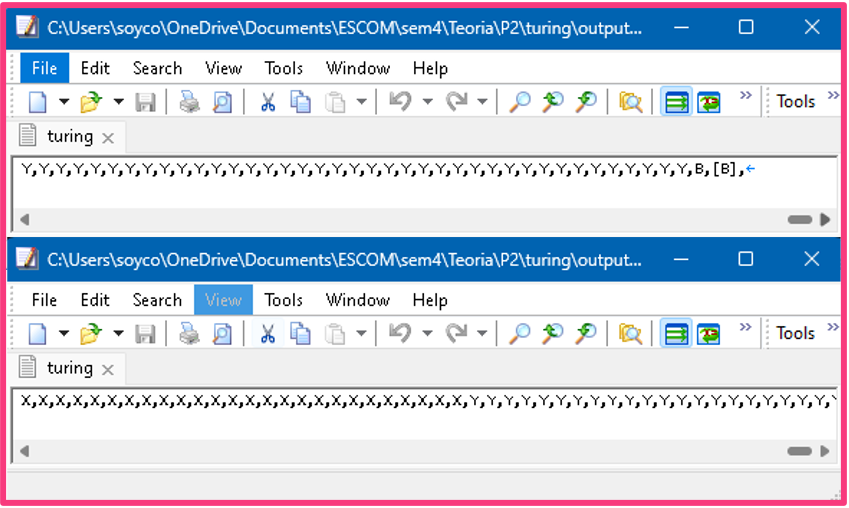
\includegraphics[width=1\linewidth]{Images/Cap7.png}
    \end{center}
%\end{minipage}
\caption{Visualización del final de archivo de salida turing.txt.}
\label{fig:imagen}
\end{figure}
\end{enumerate}
\chapter{Conclusión}
La conclusión de desarrollar y solucionar el problema de la máquina de Turing es que se trata de un modelo computacional muy poderoso y versátil. Al implementar una máquina de Turing para resolver un problema específico, se obtienen varias conclusiones:\newline
\begin{enumerate}
    \item Universalidad: La máquina de Turing es capaz de simular cualquier algoritmo computacional, lo que demuestra su capacidad para resolver problemas teóricos y prácticos de manera general.\newline
    \item Complejidad: La máquina de Turing permite analizar la complejidad de un problema al medir la cantidad de operaciones necesarias para resolverlo. Esto es fundamental para evaluar la eficiencia de los algoritmos y comprender la viabilidad de las soluciones propuestas.\newline

    \item Representación abstracta: La máquina de Turing proporciona una abstracción poderosa para representar y modelar problemas complejos. Permite separar el concepto del problema en una cinta y un cabezal que interactúa con ella, lo cual facilita el diseño de soluciones.\newline
    
    \item Limitaciones y alcance: La máquina de Turing tiene sus limitaciones, especialmente en términos de la indecibilidad de algunos problemas o la imposibilidad de resolverlos de manera eficiente. Sin embargo, también tiene un amplio alcance y puede abordar una variedad de problemas teóricos y prácticos.\newline
\end{enumerate}

En conclusión general, el desarrollo y la solución de problemas utilizando la máquina de Turing permiten comprender y analizar la computabilidad y complejidad de los problemas. Además, brindan una base sólida para el diseño y análisis de algoritmos, y ayudan a investigar los límites de lo que se puede computar.

\\

\section{Complejidades}
La complejidad tanto espacial como temporal del algoritmo dependerá fielmente del tamaño de la entrada de ceros y unos y de las reglas de transición definidas en la máquina de Turing. Pero se espera que sea un comportamiento exponencial conforme el tamaño de la entrada incremente.
\chapter{Bibliografias}
\begin{enumerate}
    \item Hopcroft, J. E., Motwani, R., & Ullman, J. D. (2006). Introduction to Automata Theory, Languages, and Computation (2nd ed.). Pearson.\newline
    \item Sipser, M. (2012). Introduction to the Theory of Computation (3rd ed.). Cengage Learning.\newline
    \item Turing, A. M. (1936). On Computable Numbers, with an Application to the Entscheidungsproblem. Proceedings of the London Mathematical Society, 42(2), 230-265.\newline
\end{enumerate}


%\textbf{Nota}: {\color{red}Revisar esta sugerencia de Segun:} %\href{https://github.com/INGEOTEC/RegionalEmbeddings}{FastText Word Embeddings for Spanish Language Variations} 


%[Objetivo: ]

\chapter{Anexos}
\lstset{
    language=C,
    basicstyle=\ttfamily\small\color{black},
    numbers=left,
    numberstyle=\tiny,
    stepnumber=1,
    numbersep=8pt,
    backgroundcolor=\color{white},
    showspaces=false,
    showstringspaces=false,
    showtabs=false,
    frame=single,
    rulecolor=\color{magenta},
    tabsize=2,
    captionpos=b,
    breaklines=true,
    breakatwhitespace=false,
    title=\lstname,
    escapeinside={\%*}{*)},
    keywordstyle=\color{blue},
    commentstyle=\color{red},
    stringstyle=\color{orange},
    morecomment=[l][\color{red}]{\#},
    otherkeywords={=,!,<,>,*,+,-,&,|,^,~},
    numbers=left,                   % Coloca los números de línea a la izquierda
    numberstyle=\tiny\color{black}, % Estilo de los números de línea
    stepnumber=1,    % Incremento en el que se muestran los números de línea
    numbersep=8pt
}
\section{Código LATEX de este documento}
Dirección GitHub:\url{https://github.com/Connor-UM-18/Teoria-Computacional---Turing.git}\newline
Dirección Overleaf:\url{https://www.overleaf.com/2428945132mnyyfwyhddjq}\newline
\section{maquina\_turing.py}
Se presenta el código implementado para la solución al problema con extensión .py . Donde es necesario tener importada la librería random y pygame. \newline
\\
\begin{lstlisting}
#Teoria de la computacion
#Maquina de turing
#Alumno: Connor Urbano Mendoza
import random
import pygame

pygame.init() #Acceso al paquete pygame
#Ancho
WIDTH = 1300
#Altura
HEIGHT = 700
screen = pygame.display.set_mode((WIDTH,HEIGHT)) #Tamanio de ventana a imprimir
pygame.display.set_caption('Maquina de turing')
font = pygame.font.Font('freesansbold.ttf',20)#Tipo de fuente 1 del juego
big_font= pygame.font.Font('freesansbold.ttf',50)#Tipo de fuente 2 del juego
timer = pygame.time.Clock()#velocidad de actualizacion de nuestro juego a 60 fps
fps=60

#Variables e imagenes del juego
ubicacion = ['recuadro']

#Variables de turnos cambiantes
turn_step = 0
selection= 100
#Cargar imagenes en juego
cuadro = pygame.image.load('C:\\Users\\soyco\\OneDrive\\Documents\\ESCOM\\sem4\\Teoria\\P2\\turing\\img\\cuadro.png')
cuadro = pygame.transform.scale(cuadro,(101,101))

cuadrado = [cuadro]

lista_piezas = ['recuadro']

#ver variables/contador flash
boton_presionado = False

def dibujar_boton():
    boton_width = 150
    boton_height = 45
    boton_x = (WIDTH - boton_width) // 2
    boton_y = (HEIGHT - boton_height - 20)-100

    # Dibujar el botón como un rectángulo en la pantalla
    boton_rect=pygame.Rect(boton_x, boton_y, boton_width, boton_height)
    pygame.draw.rect(screen, (0, 255, 0), (boton_x, boton_y, boton_width, boton_height))
    texto = font.render("Siguiente", True, (0, 0, 0))
    texto_rect = texto.get_rect(center=(boton_x + boton_width // 2, boton_y + boton_height // 2))
    screen.blit(texto, texto_rect)
    return boton_rect
   
#Funcion para dibujar el contenido de la maquina de turing
def mostrar_transiciones(recorrido,estado):
    
    #recorrido="X,0,0,1,[1],1,1,1,"
    #estado="q2"
    cuadro_size = 100  # Tamaño de cada cuadro del tablero
    x = 0
    y = 255
    
    font = pygame.font.Font(None, 100)  # Fuente y tamaño del número de casilla

    transiciones = recorrido.split(',')  # Obtener las transiciones del recorrido

    for i, transicion in enumerate(transiciones):
        if i >= 12:
            break  # Salir del bucle si se han mostrado todas las transiciones posibles
        x = x + 100
        if transicion.startswith('['):
            # Realizar alguna acción especial para la transición que comienza con '['
            # Por ejemplo, cambiar el color del recuadro o agregar un marcador adicional
            numero_texto = font.render("^", True, 'yellow')  # Crear superficie de texto con la transición
            numero_rect = numero_texto.get_rect(center=((x, y+110)))  # Posición del texto en el centro del recuadro
            screen.blit(numero_texto, numero_rect)  # Pegar el texto en la pantalla
            numero_texto = font.render("|", True, 'yellow')  # Crear superficie de texto con la transición
            numero_rect = numero_texto.get_rect(center=((x, y+120)))  # Posición del texto en el centro del recuadro
            screen.blit(numero_texto, numero_rect)  # Pegar el texto en la pantalla
            numero_texto = font.render(estado, True, 'yellow')  # Crear superficie de texto con la transición
            numero_rect = numero_texto.get_rect(center=((x, y+190)))  # Posición del texto en el centro del recuadro
            screen.blit(numero_texto, numero_rect)  # Pegar el texto en la pantalla
            index=lista_piezas.index('recuadro')
            screen.blit(cuadrado[index],(x-50,y-55))
            
        numero_texto = font.render(transicion, True, 'black')  # Crear superficie de texto con la transición
        numero_rect = numero_texto.get_rect(center=((x, y)))  # Posición del texto en el centro del recuadro
        screen.blit(numero_texto, numero_rect)  # Pegar el texto en la pantalla
 
#Funcion para dibujar tablero
def dibujar_tablero():
    cuadro_size = 100  # Tamaño de cada cuadro del tablero
    tablero_width = 12 * cuadro_size  # Ancho total del tablero
    tablero_height = 1 * cuadro_size  # Altura total del tablero
    tablero_x = (WIDTH - tablero_width) // 2  # Posición X para centrar el tablero
    tablero_y = ((HEIGHT - tablero_height) // 2 )-200 # Posición Y para centrar el tablero

    for i in range(12):  # Iterar 12 veces para un tablero de 1x12
        columna = i % 12
        fila = 1
        x = tablero_x + columna * cuadro_size
        y = tablero_y + fila * cuadro_size
        if fila % 2 == 0:
            color = 'white' if columna % 2 == 0 else (226, 255, 255)
        else:
            color = (226, 255, 255) if columna % 2 == 0 else 'white'
        pygame.draw.rect(screen, color, [x, y, cuadro_size, cuadro_size])
        pygame.draw.rect(screen, 'black', [x, y, cuadro_size, cuadro_size], 2)  # Agregar borde de color 
       
 
# Función para generar automáticamente una cadena válida
def generate_auto_string():
    n = random.randint(0, 500)
    input_string = '0' * n + '1' * n
    return input_string

def turing_M (state = None, #estados de la maquina de turing
              blank = None, #simbolo blanco de el alfabeto dela cinta
              rules = [],   #reglas de transicion
              tape = [],    #cinta
              final = None,  #estado valido y/o final
              pos = 0):#posicion siguiente de la maquina de turing

    st = state
    if not tape: tape = [blank]
    if pos <0 : pos += len(tape)
    if pos >= len(tape) or pos < 0 : 
        print("Se inicializa mal la posicion")
        SystemExit(1)
    
    rules = dict(((s0, v0), (v1, dr, s1)) for (s0, v0, v1, dr, s1) in rules)
    """
        Estado	Símbolo leído	Símbolo escrito	       Mov. 	Estado sig.
        qn(s0)  1,0,X,Y,B(v0)	  1,0,X,Y,B(v1)       R o L(dr)	   qn(s1)
    """
    while True:
        with open('C:\\Users\\soyco\\OneDrive\\Documents\\ESCOM\\sem4\\Teoria\\P2\\turing\\output\\turing.txt', 'a') as archivo:
            archivo.write(st+ '\n')
            #print (st, '\t', end=" ")
            for i, v in enumerate(tape):
                if i==pos: 
                    #print ("[%s]"%(v,),end=" ")
                    archivo.write('['+v+'],')
                else: 
                    #print (v, end=" ")
                    archivo.write(v+',') 
            #print()
            archivo.write('\n')
            if st == final: 
                print("Cadena valida.")
                break
            if (st, tape[pos]) not in rules: 
                print("Cadena invalida.")
                break
            
            (v1,dr,s1) = rules [(st, tape[pos])]
            tape[pos]=v1 #rescribe el simbolo de la cinta
    
    #movimiento del cabezal
        if dr == 'left':
            if pos > 0: pos -= 1
            else: tape.insert(0, blank)
        if dr == 'right':
            pos += 1
            if pos >= len(tape): tape.append(blank)
        st = s1

def turing_MG (state = None, #estados de la maquina de turing
              blank = None, #simbolo blanco de el alfabeto dela cinta
              rules = [],   #reglas de transicion
              tape = [],    #cinta
              final = None,  #estado valido y/o final
              pos = 0):#posicion siguiente de la maquina de turing

    st = state
    if not tape: tape = [blank]
    if pos <0 : pos += len(tape)
    if pos >= len(tape) or pos < 0 : 
        print("Se inicializa mal la posicion")
        SystemExit(1)
    
    rules = dict(((s0, v0), (v1, dr, s1)) for (s0, v0, v1, dr, s1) in rules)
    """
        Estado	Símbolo leído	Símbolo escrito	       Mov. 	Estado sig.
        qn(s0)  1,0,X,Y,B(v0)	  1,0,X,Y,B(v1)       R o L(dr)	   qn(s1)
    """
    while True:
        with open('C:\\Users\\soyco\\OneDrive\\Documents\\ESCOM\\sem4\\Teoria\\P2\\turing\\output\\turing.txt', 'a') as archivo:
            archivo.write('|-'+st+ '->')
            #print (st, '\t', end=" ")
            for i, v in enumerate(tape):
                if i==pos: 
                    #print ("[%s]"%(v,),end=" ")
                    archivo.write('['+v+'],')
                else: 
                    #print (v, end=" ")
                    archivo.write(v+',') 
            #print()
            if st == final: 
                print("Cadena valida.")
                break
            if (st, tape[pos]) not in rules: 
                print("Cadena invalida.")
                break
            
            (v1,dr,s1) = rules [(st, tape[pos])]
            tape[pos]=v1 #rescribe el simbolo de la cinta
    
    #movimiento del cabezal
        if dr == 'left':
            if pos > 0: pos -= 1
            else: tape.insert(0, blank)
        if dr == 'right':
            pos += 1
            if pos >= len(tape): tape.append(blank)
        st = s1
        
with open('C:\\Users\\soyco\\OneDrive\\Documents\\ESCOM\\sem4\\Teoria\\P2\\turing\\output\\turing.txt', 'w') as archivo:
    pass
print("Maquina de turing")
print("\n--- Menu ---")
print("1. Ingresar una cadena manualmente")
print("2. Generar una cadena automaticamente")
print("0. Salir")

option = input("Elige una opcion: ")

if option == '1':
    input_string = input("Ingrese una cadena menor a 11 caracteres. \nDigite la cadena deseada:  ")
    #se puede cambiar las reglasde transicion para otra maquina de turing
    turing_M (state = 'q0', #estado inicial de la maquina de turing
                blank = 'B', #simbolo blanco de el alfabeto dela cinta
                tape = list(input_string),#inserta los elementos en la cinta
                final = 'q4',  #estado valido y/o final
                rules = map(tuple,#reglas de transicion
                            [
                            "q0 0 X right q1".split(),
                            "q0 Y Y right q3".split(),
                            "q1 0 0 right q1".split(),
                            "q1 1 Y left q2".split(),
                            "q1 Y Y right q1".split(),
                            "q2 0 0 left q2".split(),
                            "q2 X X right q0".split(),
                            "q2 Y Y left q2".split(),
                            "q3 Y Y right q3".split(),
                            "q3 B B right q4".split(),
                            ]   
                            )
                )  
    #Animamos la maquina de turing
    #lista_estados = [int(num) for num in recorrido.split(",")]
    coordenadas=(235,85)
    nueva_coordenada=(0,0)
    run=True
    contador=1
    leerlinea=0
    with open('C:\\Users\\soyco\\OneDrive\\Documents\\ESCOM\\sem4\\Teoria\\P2\\turing\\output\\turing.txt', 'r') as archivo:
        lineas = archivo.readlines()
    
    while run:
        if len(lineas) == leerlinea:
            print("Programa termino.")
            SystemExit(0)
        timer.tick(fps)
        # Rellenar la pantalla con el color
        screen.fill((30, 22, 37))
        dibujar_tablero()
        boton_rect = dibujar_boton()
        estado = lineas[leerlinea].strip()  # Eliminar espacios en blanco al inicio y al final de la línea
        recorrido = lineas[leerlinea+1].strip()
        mostrar_transiciones(recorrido,estado)
        for event in pygame.event.get():
            if event.type == pygame.QUIT:
                run = False

            if event.type == pygame.MOUSEBUTTONDOWN and event.button == 1:
                mouse_pos = pygame.mouse.get_pos()
                if boton_rect.collidepoint(mouse_pos):  # Verificar si se hizo clic en el botón
                    leerlinea=leerlinea+2
        pygame.display.flip()
    pygame.quit()
  

elif option == '2':
    input_string = generate_auto_string()
    print("Cadena generada automaticamente:", input_string)
    print("Tamanio de cadena:", str(len(input_string)))
    turing_MG (state = 'q0', blank = 'B', tape = list(input_string),final = 'q4', rules = map(tuple,
                            #reglas de transicion
                            [
                            "q0 0 X right q1".split(),
                            "q0 Y Y right q3".split(),
                            "q1 0 0 right q1".split(),
                            "q1 1 Y left q2".split(),
                            "q1 Y Y right q1".split(),
                            "q2 0 0 left q2".split(),
                            "q2 X X right q0".split(),
                            "q2 Y Y left q2".split(),
                            "q3 Y Y right q3".split(),
                            "q3 B B right q4".split(),
                            ]   
                            )
                )
    
    
else:
    print("Opcion invalida. Inténtalo de nuevo.")
    SystemExit(0)

print("Programa termino.")

\end{lstlisting}


%\bibliographystyle{apacite}
%\bibliography{References/predoc.bib}

\backmatter%@sglvgdor


\end{document}
